\section{Selection Efficiency}
\label{sec:seleff}
%We would like to quote our results as a cross section, or cross section limit, that is as
%model independent as possible. 
%What we mean by this is that we carefully define the acceptance, and provide enough
%details about the selection efficiency within that acceptance that anybody can use their favorite Monte Carlo
%generator of new physics, define an acceptance at the hard scatter level (status = 3 in Pythia), and correctly estimate
%the efficiency for this new physics model to within 50\% or so.
%
%In the present section we provide the necessary {\em correction factors} that one needs to estimate the efficiency.
%There are three effects. 
%First, our lepton selection efficiencies vary significantly as a function of both $\pt$ and $|\eta |$,
%especially for electrons. 
%Second, both \met and $\Ht$ have {\em turn-on} curves due to finite resolution effects.
%Third, there is a potentialy significant $\pt$ dependent data/Monte Carlo scale factor that we obtain from 
%Z to dilepton events using  the tag \& probe technique.\footnote{The results of the tag \& probe measurements
%using current data and simulation suggest the difference is small and no data/MC scale factor is applied.}
%Even though the scale factors are described last, we include them in the lepton efficiency parameterization presented below
%in Section~\ref{sec:lepeff}.
%
%
%\subsection{Definition of Acceptance}
%\label{sec:acceptance}
%
%Lepton acceptance is defined for both leptons with $|\eta|<2.4$
%and with momenta either $\pt>10~\GeV$\ ($5~\GeV$) for electrons (muons) and the {\em low-\pt} dilepton selections,
%or with one lepton with $\pt > 10$\ GeV and the other with $\pt > 20$\ GeV for the {\em high-\pt} selections
%described in Section~\ref{sec:eventSel}.
%$\Ht^{\rm gen}$\ is comprised of the sum $\pt$ of all colored particles at the hard scatter level that have $\pt > 40$ GeV
%and $|\eta |<2.5$. 
%$\met^{\rm~gen}$ is defined as the absolute value of the vector sum of the transverse 
%momentum of all non-interacting particles, e.g. neutrinos and LSP.
%
%
%\subsection{Lepton Efficiencies}
%\label{sec:lepeff}
%
%These curves are to be taken directly from simulation, they are primarily relevant
%for the outside-CMS theorists to be able to use our results.
%A similar set of curves has been provided in~\cite{ref:sus10004}.
%Lepton selection efficiencies, including the MC-to-data scale factors,
%are illustrated in Fig.~\ref{fig:lepeffLM6}.
%
%\begin{figure}[h]
%\begin{center}
%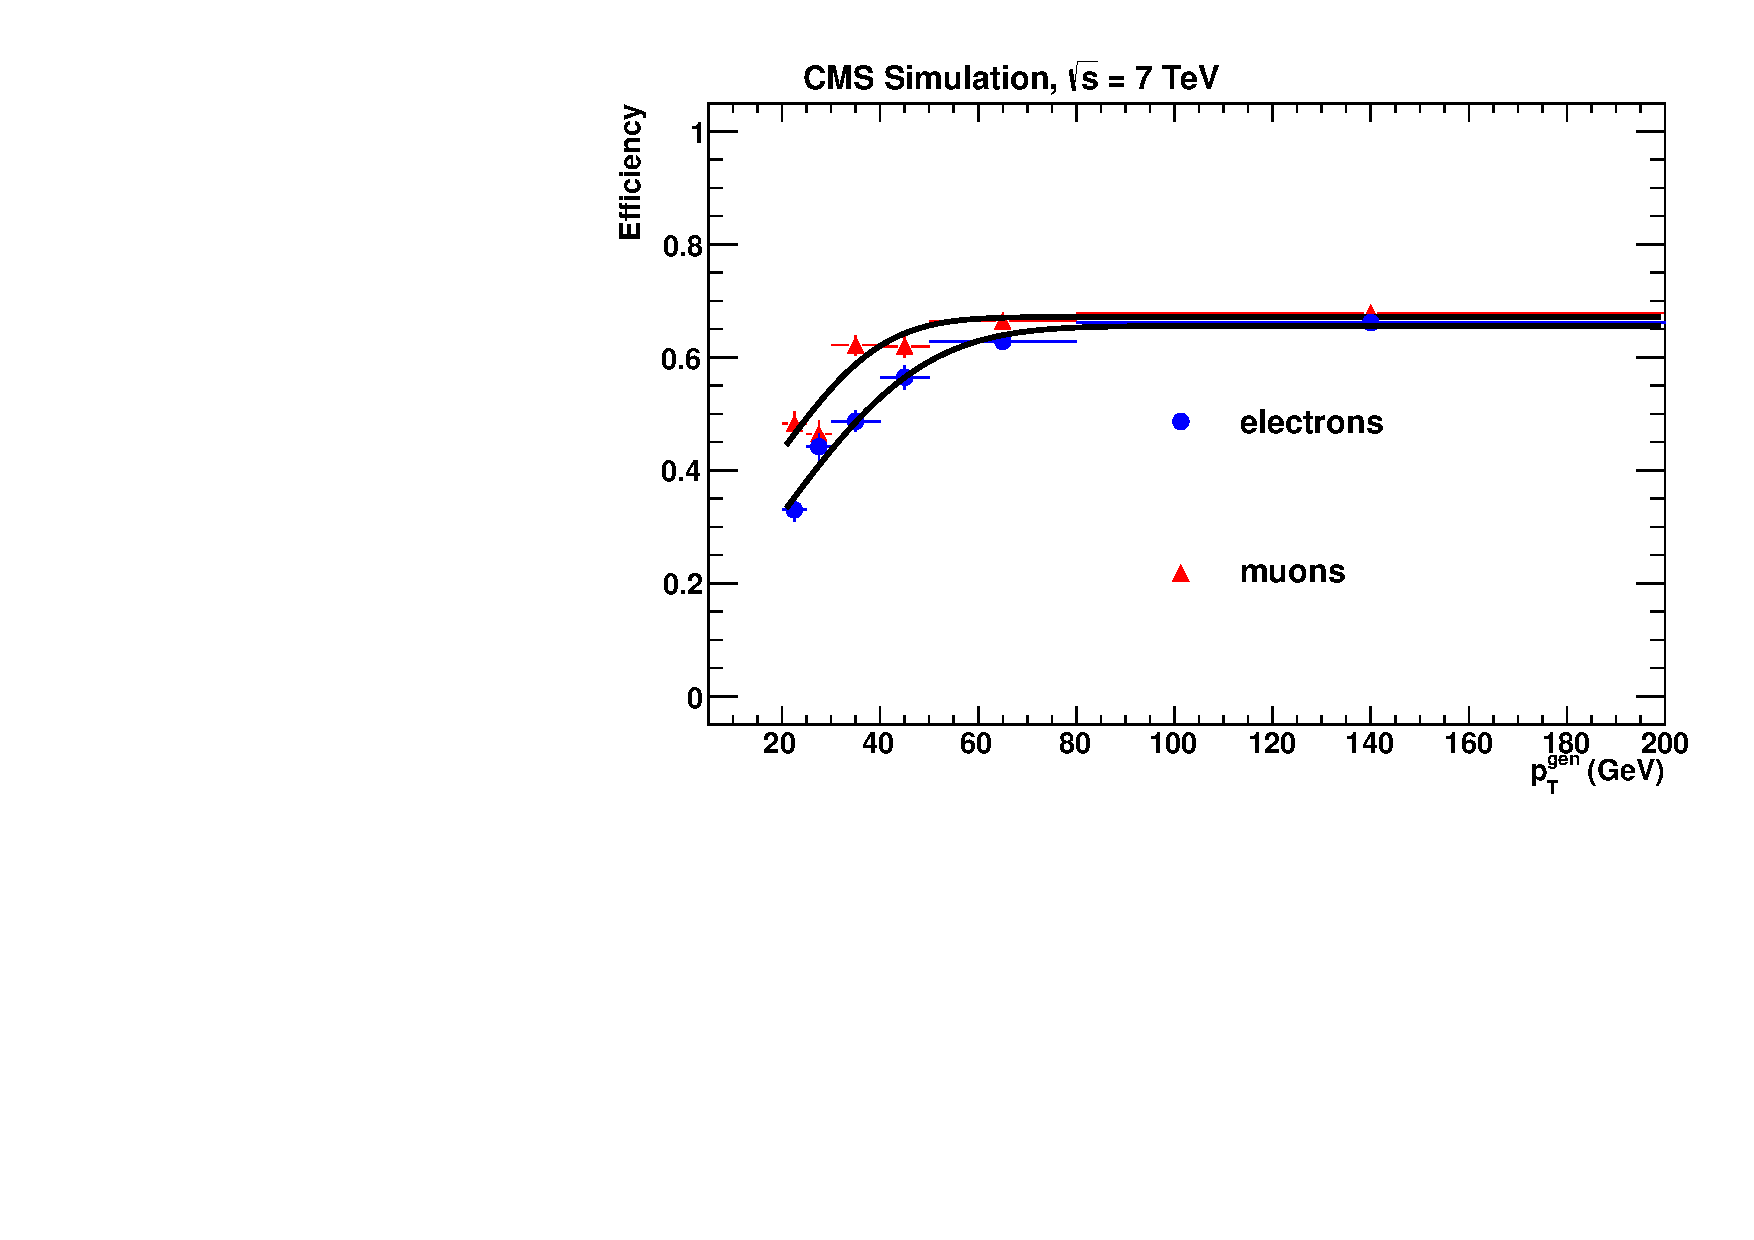
\includegraphics[width=0.7\linewidth]{figures/leptonEfficiency_lm6}
%\caption{\label{fig:lepeffLM6}
%Lepton selection efficiency as a function of \pt,
%displayed for electrons and muons.
%}
%\end{center}
%\end{figure}
%
%The efficiency dependence can be parameterzied as a function of \pt\ as 
%
%\begin{eqnarray}
%\epsilon = \epsilon_{\rm \infty} {\rm erf}\left ( \frac{\pt - C}{\sigma} \right)
%	+ \epsilon_C \left( 1.- {\rm erf}\left ( \frac{\pt - C}{\sigma} \right) \right),
%\label{eq:lepeffFitF}
%\end{eqnarray}
%where $\epsilon_{\rm \infty}$ gives the value of efficiency plateau at high momenta,
%$C$ is equal to 5 (10) for muons (electrons),
%$\epsilon_C$ gives the value of the efficiency at $\pt=C$,
%and $\sigma$ describes how fast the transition region is.
%The results of the fit for electrons and muons are summarized in Table~\ref{tab:lepeffLM6fit}.
%
%\begin{table}[h]
%\begin{center}
%\caption{\label{tab:lepeffLM6fit} Results of the fit of the dependence in Fig.~\ref{fig:lepeffLM6}
%to the function specified in Eq.~\ref{eq:lepeffFitF}.}
%\begin{tabular}{l|cc}\hline\hline
%Parameter		& Electrons		& Muons			\\ \hline
%$C$			& 10			& 5			\\
%$\epsilon_{\infty}$	& $0.721\pm0.006$	& $0.786\pm0.005$	\\
%$\epsilon_{C}$		& $0.219\pm0.017$	& $0.412\pm0.018$	\\
%$\sigma$		& $22.5\pm1.4$		& $19.5\pm1.4$		\\
%\hline\hline
%\end{tabular}
%\end{center}
%\end{table}
%
%
%
%\subsection{MET and $\Ht$ efficiency turn-on}
%\label{sec:turnon}
%Our selections on reconstructed jets begin with a requirement of at least two jets with $\pt>40~\GeV$.
%Two such jets are present in approximately 95\% of the events in LM1 and LM6 with $\Ht^{\rm gen}>200~\GeV$ prior
%to any additional requirement on colored partons at the generator level beyond the sum of \pt.
%This represents the fraction of acceptance to two jets.
%In the following we proceed with determining $\Ht$ amd \met\ requirement with respect to 
%events that have generator-level requirements on the leptons and colored particles as described in Section~\ref{sec:acceptance}.
%
%The efficiency for an event to pass a given reconstructed \met\ ($\Ht$) threshold is shown in Fig.~\ref{fig:htmetThresh}
%as a function of $\met^{\rm~gen}$ ($\Ht^{\rm gen}$) in events passing $\Ht^{\rm gen}>200~\GeV$ ($\met^{\rm~gen}>30~\GeV$).
%Due to rather small fraction of events in LM6 simulation having low \Ht\ activity, the \Ht\ curves are made with LM1.
%Results of the fits of these curves to $0.5 \epsilon_{\infty} \{{\rm erf}[(x - x_{1/2})/\sigma] + 1\}$ are summarized
%in Table~\ref{tab:htmetThresh}.
%Neither the \met\ nor \Ht\ curves show a significant bias in the position of the point with half the plateau efficiency ($x_{1/2}$).
%The inefficiency at the plateau is essentially negligible.
%The width of the threshold $\sigma$ increases with the value of the cut.
%
%\begin{figure}[h]
%\begin{center}
%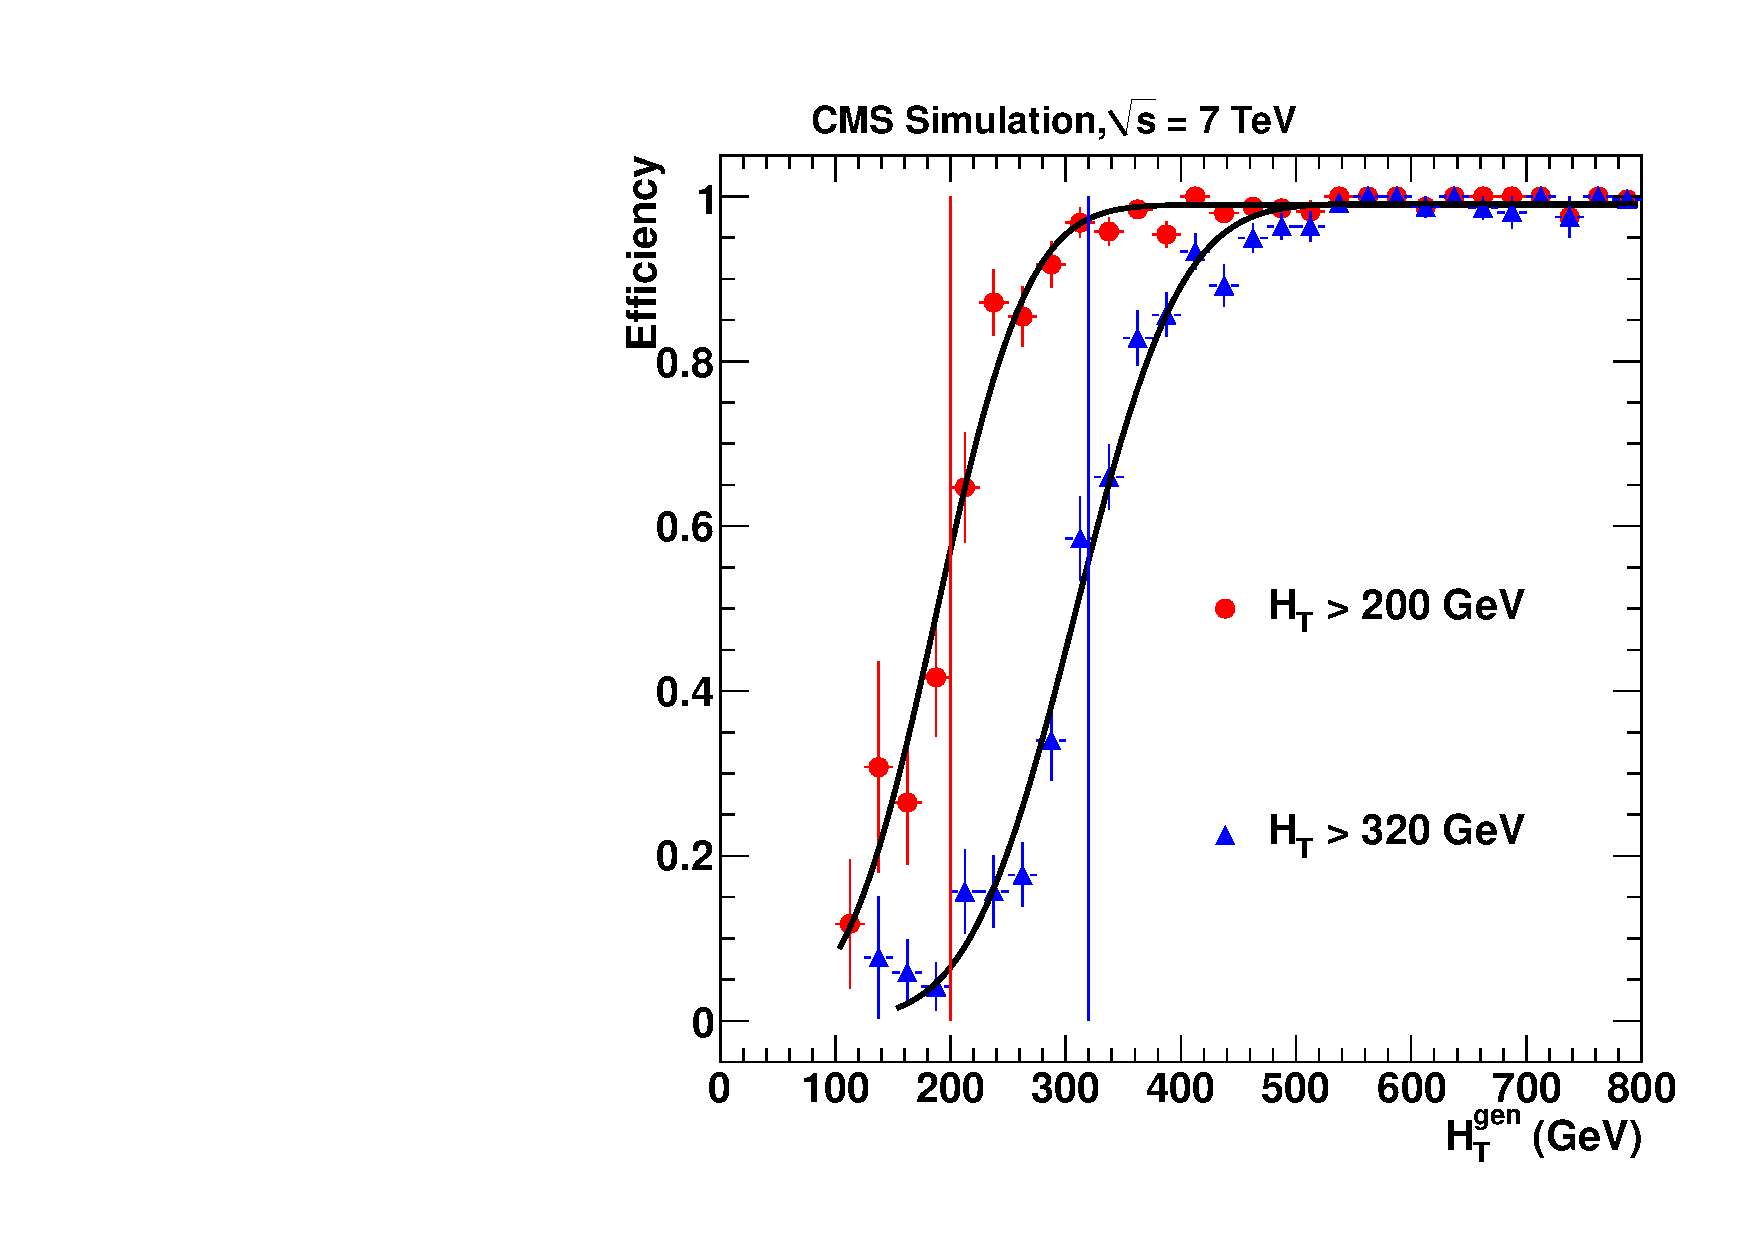
\includegraphics[width=0.48\linewidth]{figures/HTturnOnCurve_lm1}
%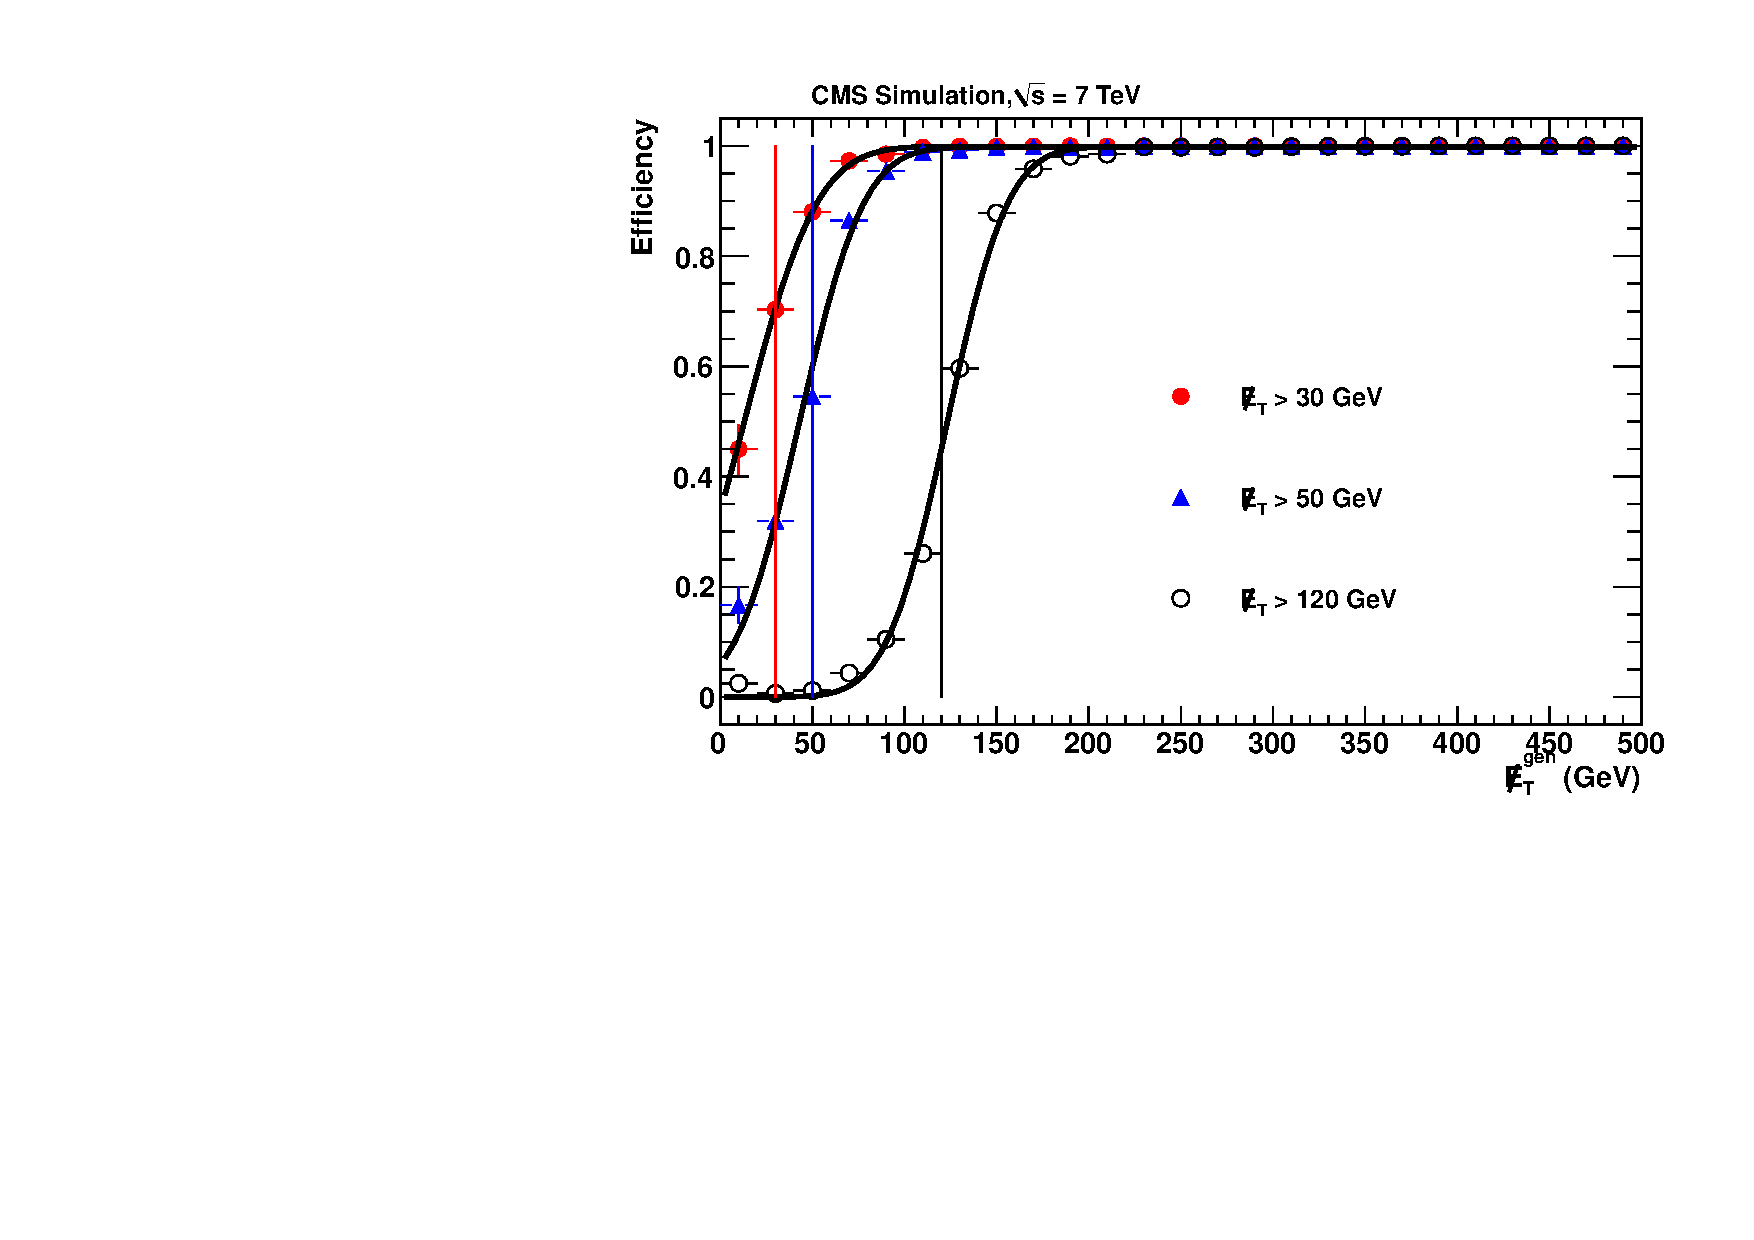
\includegraphics[width=0.48\linewidth]{figures/metTurnOnCurve_lm6}
%\caption{\label{fig:htmetThresh}
%Efficiency for an event to pass a given reconstructed \met\ ($\Ht$) threshold 
%as a function of $\met^{\rm~gen}$ ($\Ht^{\rm gen}$).
%The curves are shown for \met\ thresholds of 50, and 120~\GeV;
%the thresholds for \Ht\ are 200, and 450~\GeV.
%}
%\end{center}
%\end{figure}
%
%
%\begin{table}[h]
%\begin{center}
%\caption{\label{tab:htmetThresh} Results of the fit of the dependence in Fig.~\ref{fig:htmetThresh}
%to $0.5 \epsilon_{\infty} \{{\rm erf}[(x - x_{1/2})/\sigma] + 1\}$.}
%\begin{tabular}{l|cc|cc}\hline\hline
%Parameter		& \multicolumn{2}{|c}{\Ht}			& \multicolumn{2}{|c}{\met}			\\ 
%			&	$>200~\GeV$	& $> 450~\GeV$		& $>50~\GeV$		& $>120~\GeV$	\\ \hline
%$\epsilon_{\infty}$	& $0.997\pm0.001$	& $0.992\pm0.001$	& $0.999\pm0.001$	& $0.999\pm0.001$ \\
%$x_{1/2}$		& $185.4\pm 4.0$	& $440.6\pm1.8$		& $43.0\pm1.1$		& $123.3\pm 0.5$  \\
%$\sigma$		& $99.2\pm6.0$		& $120.3\pm3.4$		& $38.9\pm1.6$		& $36.6\pm0.9$	\\
%\hline\hline
%\end{tabular}
%\end{center}
%\end{table}


\subsection{Data - Monte Carlo Scale Factor for Leptons}
\label{sec:tnp}

The efficiencies of the lepton isolation and identification requirements (including all quality requirements) 
are measured with the tag\&probe method in dilepton Z events using the full 2011 dataset.
The efficiency of the identification requirements is a property of the lepton itself and is directly applicable
 to the leptons in signal events.
The efficiency of the isolation requirement, however, is a strong function of all other (mainly hadronic)
activity in the event.
The following results are based on measurements using the full dataset and compared 
to simulation that is re-weighed to have a pile-up distribution comparable to that observed in data.

The electron selection efficiencies are measured in events passing 
the \verb=Ele17..._SC8_Mass30= and \\\verb=Ele17.._Ele8_Mass30= triggers,
which require one well-identified electron and one super-cluster or GSF electron with $\pt>8~\GeV$ forming a pair with a mass
above 30~\GeVcc.  
For higher $\pt$ electrons, the \verb=Ele32...SC_17= triggers are also used, 
which require one well identified electron and one super-cluster with $\pt >17~\GeV$.
In the tag\&probe analysis the electron tag is required to match to the well-identified electron 
from the trigger and also to pass all the electron requirements described in~\cite{ssnote2011}.
The probe electron is required to have
\begin{itemize}
\item $\pt>20~\GeV$, $|\eta|<2.4$, excluding the superclusters with $1.4442<|\eta|<1.566$.
\end{itemize}
The isolation efficiency is measured with the probes passing all electron selections , except for the 
trigger requirement and the isolation itself.
The identification efficiency is measured with probes passing the isolation requirement.
Results of the measurement are summarized in Table~\ref{tab:eleEffs}.
The contribution from the Z events is based on simple counting in the mass range of 86--96~\GeVc,
the MC contribution includes Wjet events to match the expected residual backgrounds in this mass window.
The following sources of systematic uncertainty are attributed to this measurement:
background contribution, selection of dielectron events, factorization of the isolation and ID parts.
The size of the background contribution can be estimated using MC alone
and also  tested in data with  the same-sign dielectron
events, which should represent the number of backgrounds reasonably well.
The effect of backgrounds on the measured efficiency is established to be approximately 
2\% for the combined identification
and isolation selection efficiency.
The narrow mass window used to count electron pairs introduces a bias of about 3\% 
to the measured efficiency
by rejecting failing probes that happen to have a worse resolution or a shift
in the measured momentum.
This bias is expected to approximately cancel in data and simulation.
We include a half of the 3\% as a source of systematics.
Based on simulation alone, the combined selection efficiency, measured with respect to the probe electron,
differs from the product of the components by approximately 1\% or less depending on the momentum range.
All of these effects combined give a systematic uncertainty on the total data-to-MC scale factor
in the lepton selection efficiencies of 2.5\% for $\pt>20~\GeV$.

\begin{table}[h]
\begin{center}
\begin{tabular}{c|c|ccc}
\hline\hline
& & 20 - 40 GeV & 40 GeV -  \\
\hline
				& MC			& 	0.9268 $\pm$ 0.0004 & 	0.9768 $\pm$ 0.0002 \\
ISO				& DATA			& 	0.9247 $\pm$ 0.0003 & 	0.9737 $\pm$ 0.0002 \\
				& DATA/MC		& 	0.9977 $\pm$ 0.0005 & 	0.9968 $\pm$ 0.0003 \\
\hline
				& MC			& 	0.8069 $\pm$ 0.0005 & 	0.8500 $\pm$ 0.0004 \\
ID				& DATA			& 	0.8005 $\pm$ 0.0005 & 	0.8343 $\pm$ 0.0004 \\
				& DATA/MC		& 	0.9921 $\pm$ 0.0008 & 	0.9815 $\pm$ 0.0006 \\
\hline
				& MC			& 	0.7478 $\pm$ 0.0005 & 	0.8303 $\pm$ 0.0004 \\
ID X ISO			& DATA			& 	0.7403 $\pm$ 0.0005 & 	0.8124 $\pm$ 0.0004 \\
				& DATA/MC		& 	0.9899 $\pm$ 0.0010 & 	0.9784 $\pm$ 0.0007 \\
\hline \hline
\hline
\end{tabular}
\caption{\label{tab:eleEffs}Electron isolation and identification efficiencies measured with the tag\&probe method.
The uncertainties are statistical only.}
\end{center}
\end{table}

The muon selection efficiencies are measured using events passing the double-muon trigger.
The tag muon is required to pass all of the muon selection requirements described in~\cite{ssnote2011}.
The probe muon is required to pass
\begin{itemize}
\item $\pt>20~\GeVc$;
\item $|\eta|<2.4$;
\item have both the global and the tracker muon types.
\end{itemize}
Both the  isolation and the identification efficiency are measured using probes failing only the requirement in question,
assuming the efficiencies factorize.
Results of the muon identification and isolation efficiency measurements are presented in Table~\ref{tab:muEffs}.
As expected, the identification efficiency for muons measured in data and in MC agree well,
while there is some discrepancy for the isolation efficiency.
Similar sources of systematic uncertainty are considered here as those considered for electrons.
Most of the reconstructed (probe) muons are real muons and the measurement of the identification efficiency
is not affected significantly by backgrounds.
With the tighter mass window used here to select events,
 the backgrounds are estimated to be small.
This narrow mass window, however, introduces a bias of about 1.5\% 
to the measured efficiency
by rejecting failing probes that happen to have a worse resolution or a shift
in the measured momentum.
This bias is expected to approximately cancel in data and simulation.
We include a half of the 1.5\% as a source of systematics.
We assign a systematic uncertainty of 1\% on the identification and isolation efficiency measurement  
from a comparison between the simple counting of Z events and fitting the mass shape to a gaussian signal and an 
exponential background component.
Based on studies in MC events, we find that the isolation and the identification efficiencies
 factorize near-perfectly and do not assign any additional systematic uncertainty.
The total systematic uncertainty on the muon efficiency measurement in 
data, simply covering the full momentum range, is 2\%.


\begin{table}[h]
\begin{center}
\begin{tabular}{c|c|cc}
\hline\hline
& & 20 - 40 GeV & 40 GeV -  \\ 
\hline
				& MC			& 	0.9111 $\pm$ 0.0003& 	0.9747 $\pm$ 0.0002 \\
ISO				& DATA			& 	0.8969 $\pm$ 0.0003& 	0.9668 $\pm$ 0.0002 \\
				& DATA/MC		& 	0.9844 $\pm$ 0.0004& 	0.9919 $\pm$ 0.0002 \\
\hline
				& MC			& 	0.9710 $\pm$ 0.0002& 	0.9612 $\pm$ 0.0002 \\
ID				& DATA			& 	0.9666 $\pm$ 0.0002& 	0.9561 $\pm$ 0.0002 \\
				& DATA/MC		& 	0.9955 $\pm$ 0.0003& 	0.9947 $\pm$ 0.0003 \\
\hline
				& MC			& 	0.8847 $\pm$ 0.0003& 	0.9369 $\pm$ 0.0002 \\
ID X ISO			& DATA			& 	0.8669 $\pm$ 0.0003& 	0.9244 $\pm$ 0.0002 \\
				& DATA/MC		& 	0.9799 $\pm$ 0.0005& 	0.9866 $\pm$ 0.0003 \\
\hline \hline
\end{tabular}
\caption{\label{tab:muEffs}Muon isolation and identification efficiencies measured with the tag\&probe method.
The uncertainties are statistical only.}
\end{center}
\end{table}

The tag\&probe results in Tables~\ref{tab:eleEffs} and~\ref{tab:muEffs}
show that for leptons with $\pt>20~\GeV$ used in this analysis both the ID part and the isolation parts
 of the lepton selection are reproduced well by simulation, already within the systematic uncertainties
quoted above.
Application of this measurement based on Z events to the signal events incurs
an additional uncertainty due to potential mismodeling of the isolation requirement.
In agreement with Ref.~\cite{ssnote2011}, we assign a systematic uncertainty of 5\% 
due to modeling of the isolation efficiency for signal events.
Considering the small size of the difference between data and simulation reported in 
Tables~\ref{tab:eleEffs} and~\ref{tab:muEffs}, compared to the systematic uncertainty
applicable to the analysis,
we approximate the scale factor to be 1.0 for both simulated signal and backgrounds
and propagate the uncertainty described above to the relevant part of the analysis
(signal selections) described in Section~\ref{sec:systematic}.

\subsection{Data - Monte Carlo Scale Factor for b-jets}
\label{sec:bjetSF}
We apply an average scale factor of 0.96 measured using \ttbar\ events
for the SSVHEM tagger~\cite{BTV11003}.
The uncertainty on the scale factor is 4 (15)\% for jets with $\pt<240 (>240)~\GeV$,
as recommended by the b-tagging POG~\cite{btvSyst} and apply
it to the analysis as described in Section~\ref{sec:systematic}.